% Created 2019-12-16 Mon 23:03
% Intended LaTeX compiler: pdflatex
\documentclass[11pt]{article}
\usepackage[utf8]{inputenc}
\usepackage[T1]{fontenc}
\usepackage{graphicx}
\usepackage{grffile}
\usepackage{longtable}
\usepackage{wrapfig}
\usepackage{rotating}
\usepackage[normalem]{ulem}
\usepackage{amsmath}
\usepackage{textcomp}
\usepackage{amssymb}
\usepackage{capt-of}
\usepackage{hyperref}
\usepackage{minted}
\author{Tigany Zarrouk\thanks{tigany.zarrouk@skf.com}}
\date{25.11.2019}
\title{Atomistic investigation of dislocation assisted C migration in Dark Etching Regions}
\hypersetup{
 pdfauthor={Tigany Zarrouk},
 pdftitle={Atomistic investigation of dislocation assisted C migration in Dark Etching Regions},
 pdfkeywords={},
 pdfsubject={},
 pdfcreator={Emacs 26.3 (Org mode 9.1.9)}, 
 pdflang={English}}
\begin{document}

\maketitle



\section*{Motivation}
\label{sec:orgb765987}
\begin{itemize}
\item Carbon redistribution and plastic deformation are thought to be
fundamental mechanisms behind DER formation.
\item Differing mechanisms of dislocation-driven carbon migration have
been suggested, but no consensus.
\item Atomistic modelling necessary to elucidate how dislocations could
move carbon; thus clarifying potential mechanisms of DER
formation.
\end{itemize}

\section*{Aims}
\label{sec:orgfe7d825}
To answer the questions:
\begin{itemize}
\item How do dislocations assist carbon migration?
\item How are dislocations influenced by carbon on atomistic scale?
\begin{itemize}
\item How does carbon affect kink-pair nucleation/migration?
\item How fast do the dislocations move in carbon environment?
\item What dislocation structures are found with dislocation movement?
\end{itemize}
\end{itemize}

\section*{Methods}
\label{sec:orgc3e048c}

\subsection*{Tight Binding}
\label{sec:orgc72b5dd}


\begin{itemize}
\item Tight binding is an approximation to DFT.
\item Overlaps between atomic orbitals are key parameters.
\item Parameters can be fitted to experimental data.
\item \(\mathcal{O}(N^3)\), but much smaller prefactor compared to DFT.
\end{itemize}

\subsection*{Line Tension Model}
\label{sec:orga25c5e9}


\begin{itemize}
\item Line Tension model approximates energy along core dislocation
dislocation line.
\item Parameters derived from atomistics: Peierls barrier (\(\Delta
  E_{\text{P}}\)), \(K\), \(\Delta E_{\text{C}}\).

\item Defined as

\(E^{\text{LT}} = \frac{K}{2}\sum_j(P_j + P_{j + 1})^2 + \sum_j  E_\text{P}(\mathbf{P}_j) + \big{ (\sigma \otimes \mathbf{b}) \times \mathbf{l} \big} \cdot  \mathbf{P_j} - \sum_{j,k} E_{\text{C}(  \mathbf{P}_j - \mathbf{P}_k^{\text{C}} )\)
\end{itemize}


[1] Itakura, M., \emph{et al.},  Acta Materialia (2013).  


\subsection*{Kinetic Monte Carlo}
\label{sec:orgd0d23af}


\begin{itemize}
\item kMC simulations model the movement of dislocations on much larger
timescales than atomistics.
\item Propogation of dislocation line segments are treated as rare events
with particular rates and mechanisms depending on local environment.
\item Rates for each of the mechanism are derived from atomistic
calculations.
\item One can find dislocation velocity as a function of stress and
temperature.
\end{itemize}
\subsection*{Summary of Methods}
\label{sec:org4b4544b}
\begin{itemize}
\item Tight-binding simulations to determine influence of carbon on
dislocations and for line-tension model constants.
\item Line tension model of dislocation to acquire stress-dependent
kink-pair formation energies.
\item Kinetic Monte Carlo model of dislocations in carbon environment to
ascertain behaviour of dislocations in carbon environment.
\end{itemize}
\begin{center}
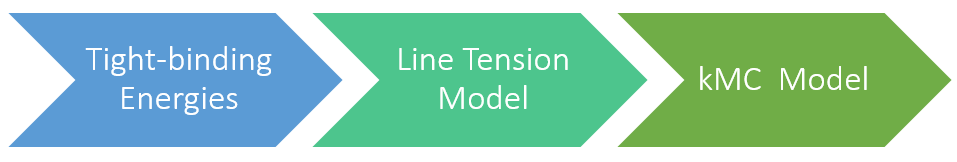
\includegraphics[width=.9\linewidth]{/home/tigany/Documents/docs/Management/Images/skf_process_tb_lt_kmc.PNG}
\label{org1cc9a54}
\end{center}
\section*{Plan}
\label{sec:org80a39e4}

\uline{Tight-binding:}
\begin{enumerate}
\item C/defect solution energies
\begin{enumerate}
\item In perfect lattice
\item With dislocation
\end{enumerate}
\item Dislocation core reconstruction with C
\item Constants for line tension model.
\end{enumerate}

\uline{Line-tension model:}
\begin{enumerate}
\item Kink-pair formation energies
\begin{enumerate}
\item Without C
\item With C in different interstitial sites
\item Under stress
\end{enumerate}
\item kMC transition rates
\end{enumerate}

\subsection*{Gantt Chart}
\label{sec:org2377a52}
\begin{center}
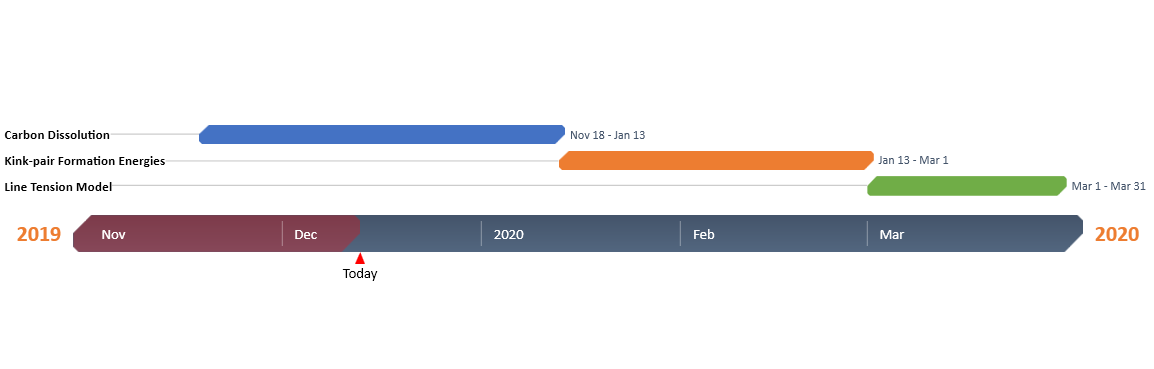
\includegraphics[width=.9\linewidth]{/home/tigany/Documents/docs/Management/Images/skf_gantt_chart_der_project_updated_larger.PNG}
\label{orga6932ab}
\end{center}


\section*{Summary}
\label{sec:org1baab26}
\begin{itemize}
\item Dislocation-assisted carbon migration thought to be fundamental
mechanism behind DER formation.
\item No consensus on which mechanism is correct, if it is at all the case.
\item Simulations can give insight into how dislocations interact with
carbon, thus elucidating potential mechanism.

\item Tight-binding can be used to model energetics of carbon and
dislocations and constants for line-tension model.
\item Line-tension model can obtain kink-pair formation energies for kMC
model.
\item kMC model can be used to see dislocation behaviour on longer
length and timescales, allowing for us to elucidate mechanisms of
dislocation-assisted carbon migration.
\end{itemize}
\section*{References}
\label{sec:org9141a66}
\end{document}